\documentclass[twoside,a4paper]{article}
\usepackage{geometry}
\geometry{margin=1.5cm, vmargin={0pt,1cm}}
\setlength{\topmargin}{-1cm}
\setlength{\paperheight}{29.7cm}
\setlength{\textheight}{25.3cm}

% useful packages.
\usepackage{amsfonts}
\usepackage{amsmath}
\usepackage{amssymb}
\usepackage{amsthm}
\usepackage{enumerate}
\usepackage{graphicx}
\usepackage{multicol}
\usepackage{fancyhdr}
\usepackage{layout}
\usepackage[UTF8]{ctex}
\usepackage{booktabs}
\usepackage{float}
\usepackage{subfigure}

% some common command
\newcommand{\dif}{\mathrm{d}}
\newcommand{\avg}[1]{\left\langle #1 \right\rangle}
\newcommand{\difFrac}[2]{\frac{\dif #1}{\dif #2}}
\newcommand{\pdfFrac}[2]{\frac{\partial #1}{\partial #2}}
\newcommand{\OFL}{\mathrm{OFL}}
\newcommand{\UFL}{\mathrm{UFL}}
\newcommand{\fl}{\mathrm{fl}}
\newcommand{\op}{\odot}
\newcommand{\Eabs}{E_{\mathrm{abs}}}
\newcommand{\Erel}{E_{\mathrm{rel}}}

\begin{document}

\pagestyle{fancy}
\fancyhead{}
\lhead{陈越 (22035026)}
\chead{学习报告}
\rhead{2023/2}

\section*{1. 问题描述}
给定一个长时间序列$X^{*}$,在t时刻,时间序列预测就是基于过去的T步$X_{t-T+1:t} = \{ x_{t - T + 1},...,x_{t} \} $去预测未来的$\tau$步$\hat{X}_{t+1:t+\tau} = \{ \hat{x}_{t + 1},...,\hat{x}_{t + \tau} \} $。这里,T和$\tau$分别是回溯窗口长度和预测窗口长度,$x_{t} \in R^d$是t时刻序列的真实值,$\hat{x}_{t} \in R^d$是t时刻的预测值,d是序列的特征维度(在目前的讨论中,d默认为1)。

\section*{2. 相关工作}
现如今已经有了许多时序预测模型,我们第一步做的工作就是对于现有的时序预测模型的效果进行评估。我们已评估的模型有Transformer、Informer、Autoformer、SCINet、Cost、FEDformer和DLinear。评估的数据集包含电力、天气、金融等多个领域,我们将每个数据集按照7:1:2的比例划分,即将70\%的数据作为训练集,10\%的数据作为验证集,20\%的数据作为测试集。模型的评估指标主要是观察测试集上的mse(均方误差)和mae(平均绝对误差),它们的具体定义如下:

\begin{equation}
    mse = \frac{1}{N} \sum_{i=1}^{N} ( x_{i} - \hat{x}_{i} )^2
\end{equation}

\begin{equation}
    mae = \frac{1}{N} \sum_{i=1}^{N} | x_{i} - \hat{x}_{i} |
\end{equation}

\noindent 其中,N是测试集的样本个数。对于同一个数据集,模型的mse和mae越小,说明模型的预测精确度越高。\par

评估的结果如下所示:\par

\begin{table}[h]
    \centering
    \scalebox{0.8}{
    \begin{tabular}{ccccccccccccccc}
    \hline
    模型 & \multicolumn{2}{c}{Transformer} & \multicolumn{2}{c}{Informer} & \multicolumn{2}{c}{Autoformer} & \multicolumn{2}{c}{SCINet} & \multicolumn{2}{c}{Cost} & \multicolumn{2}{c}{FEDformer} & \multicolumn{2}{c}{DLinear}  \\
    \cmidrule(lr){2-3} \cmidrule(lr){4-5} \cmidrule(lr){6-7} \cmidrule(lr){8-9}
    \cmidrule(lr){10-11} \cmidrule(lr){12-13}
    \cmidrule(lr){14-15}
    度量 & mse & mae & mse & mae & mse & mae & mse & mae & mse & mae & mse & mae & mse & mae \\
    \hline
    ETTh1 & 7.836 & 2.256 & 9.702 & 2.569 & 6.099 & 1.894 & 4.838 & 1.688 & 3.353 & 1.382 & 3.120 & 1.350 & \textbf{2.618} & \textbf{1.197} \\
    Weather & 43.30 & 5.111 & 25.79 & 4.386 & 8.269 & 2.256 & 6.306 & 1.926 & 85.83 & 8.082 & 5.776 & 1.859 & \textbf{5.362} & \textbf{1.740} \\
    SSE & 16237 & 98.37 & 21225 & 114.4 & 30685 & 113.1 & 14356 & 86.31 & 16541 & 96.02 & 14376 & 87.38 & \textbf{13633} & \textbf{85.93} \\
    Linear & 306544 & 468.4 & 2058923 & 1345 & 5.294 & 1.608 & 10.83 & 2.645 & 7889 & 75.77 & 0.641 & 0.556 & \textbf{0.0001} & \textbf{0.0005} \\
    Sin & 0.0015 & 0.0354 & 0.0013 & 0.0320 & 0.0017 & 0.0334 & 0.0004 & 0.0152 & 0.0001 & 0.0059 & 0.0001 & 0.0051 & \textbf{0.0001} & \textbf{0.0002} \\
    Trend & 176.6 & 8.955 & 436.7 & 16.51 & 194.9 & 10.60 & \textbf{0.766} & \textbf{0.588} & 654.7 & 20.89 & 215.3 & 13.02 & 268.4 & 14.15 \\
    Season & 0.292 & 0.399 & 0.583 & 0.636 & 8.940 & 2.194 & \textbf{0.049} & \textbf{0.146} & 0.664 & 0.574 & 0.156 & 0.275 & 0.767 & 0.587 \\
    \hline
    \end{tabular}
    }
    \caption{现有模型的单变量时间预测结果。其中Weather数据集上回溯窗口和预测窗口长度都为96,而其它数据集上回溯窗口长度为48,预测窗口长度为24。最好的结果已\textbf{加粗}。}
\end{table}

\section*{3. 模型改进}
从上述的评估结果,我们发现在大部分数据集上,简单的DLinear模型表现的效果反而最好,但当面临人为构造的复杂趋势(Trend)和周期(Season)数据集时,它的表现效果就不如SCINet了。因此我们想法便是借鉴DLinear和SCINet模型的思想去构造一个新的模型DLSResnet,主要是采用深度分解架构和Resnet结构来捕获时间序列的特征,暂时模型的整体框架如下图所示:\par

\begin{figure}[H]
\centering 
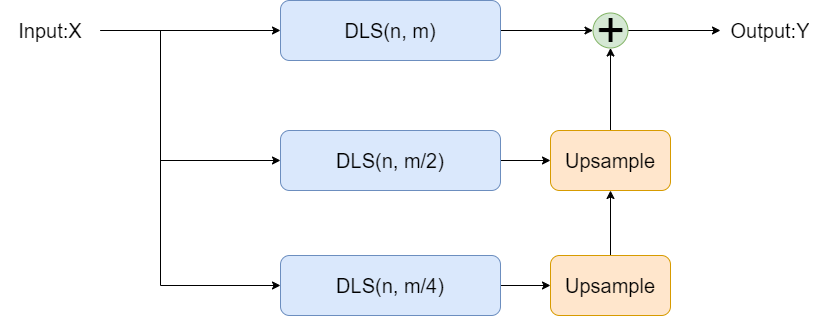
\includegraphics[width=0.8\textwidth]{model1.png} 
\caption{模型整体架构。其中DLS(n,m)是深度分解架构,n代表输入序列长度,m为输出序列长度,Upsample是上采样操作。}
\end{figure}

\subsection*{3.1 深度分解架构}
Autoformer相比于Informer模型的一大优点便是采用了趋势周期分解架构,即作者认为对于时间序列而言,将它的趋势和周期项分离开来可能对模型的预测更有效。可是若一开始便将序列进行分解,并将分解的趋势和周期项放入不同的模型中去预测,那么最后的预测效果将极大的取决于之前的分解效果。为了避免这一情况的发生,我们借鉴Autoformer的思想将序列分解架构贯彻到模型中去,具体的做法如下图所示:

\begin{figure}[H]
\centering 
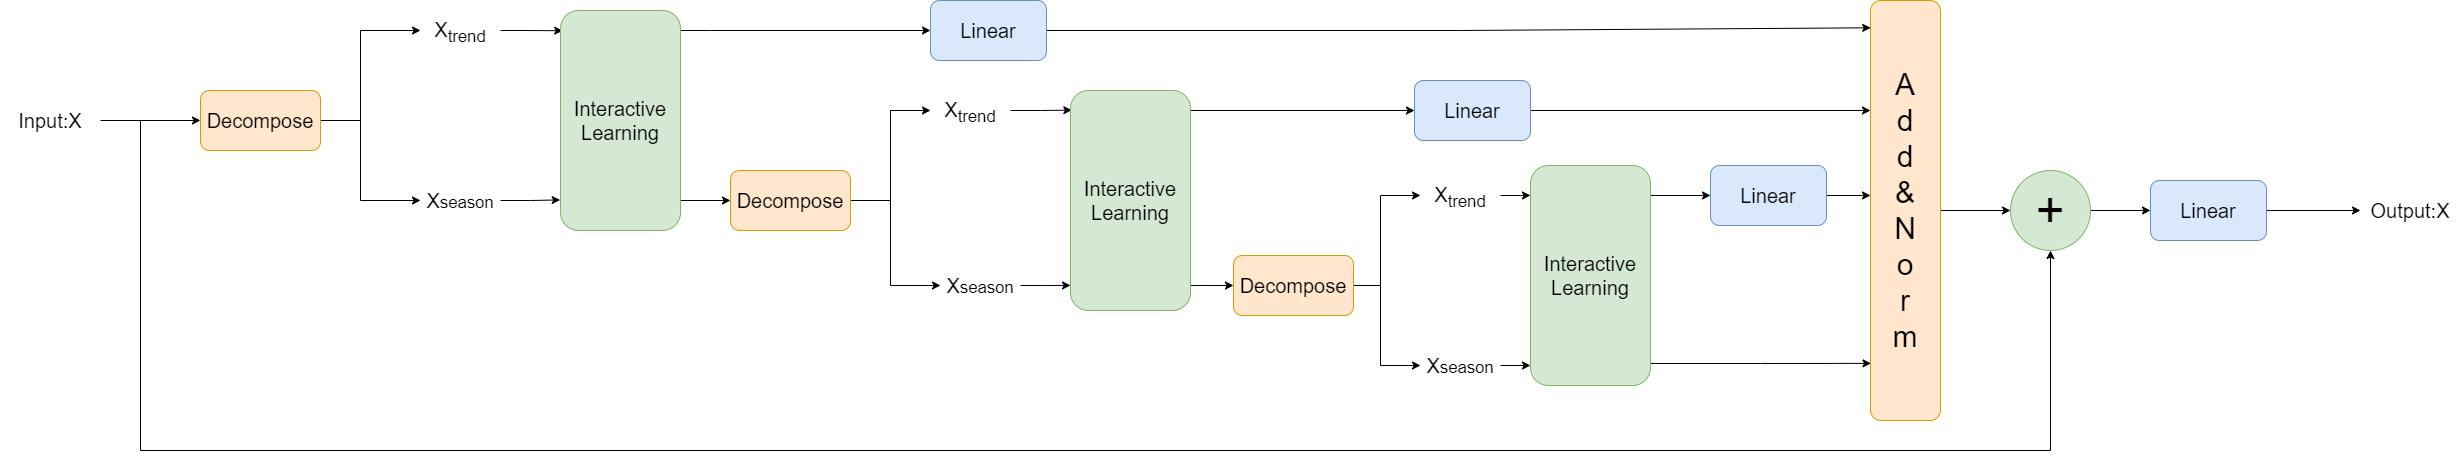
\includegraphics[width=1\textwidth]{DLS_internal.png} 
\caption{深度分解架构。其中Decompose模块是进行解耦合操作,用来分离序列的趋势项和周期项,Interactive Learning模块是SCINet中的SCI-Block,主要是让分离出来的周期项和趋势项进行交互,Linear是一个简单的线性层。}
\end{figure}

\subsubsection*{3.1.1 Decompose}
目前主流的趋势-周期分解方式主要有三种:移动平均(Autoformer)、混合专家(FEDformer)和多项式拟合。上述的三种分解方式我们都做过了测试,总体而言对模型的预测精度影响不大,因此我们这里主要介绍移动平均方法,这也是本文所用到的序列分解方式:\par

\begin{equation}
    X_{trend} = AvgPool(Padding(X))
\end{equation}

\begin{equation}
    X_{season} = X - X_{trend}
\end{equation}

\subsubsection*{3.1.2 Interactive Learning}

对于已经分离出来的趋势项和周期项,我们将其输入到Interactive Learning模块中进行交互。具体的操作是通过卷积模块$\phi$和$\psi$分别提取趋势和周期特征,并将提取到的特征通过exp函数,然后进行哈达玛积。这可以看作是在趋势和周期项上进行缩放变换,其中使用神经网络模块相互学习缩放因子。

\begin{equation}
    X_{trend}^s = X_{trend} \odot exp(\phi(X_{season})) , \quad
    X_{season}^s = X_{season} \odot exp(\psi(X_{trend}))
\end{equation}

\begin{equation}
    X_{trend}^{'} = X_{trend}^s + \rho(X_{season}^s)
    , \quad
    X_{season}^{'} = X_{season}^s + \eta(X_{trend}^s)
\end{equation}

然后,正如公式(6)所示,两个缩放后的项$X_{trend}^s$和$X_{season}^s$通过卷积模块$\rho$和$\eta$进一步提取特征并将它们分别加到$X_{season}^s$和$X_{trend}^s$上,最后输出$X_{trend}^{'}$和$X_{season}^{'}$。卷积模块$\phi$、$\psi$、$\rho$和$\eta$的结构如下所示,首先会通过复制填充来减少卷积运算的边界效应,然后采用核大小为k的一维卷积将特征维度由C扩展到h$*$C,进而进行LeakyRelu和Dropout,然后再使用一个一维卷积层将特征维度恢复到C,最后经过Tanh激活函数。

\begin{figure}[H]
\centering 
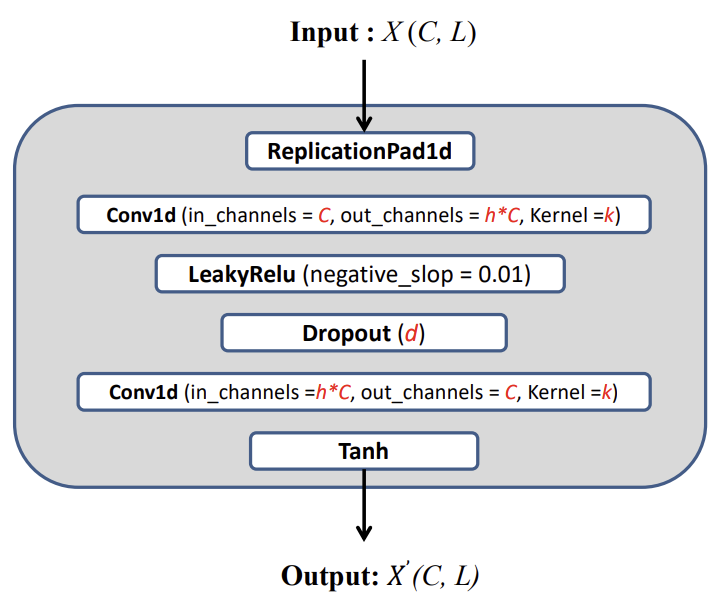
\includegraphics[width=0.4\textwidth]{SCINet.png} 
\caption{$\phi$、$\psi$、$\rho$和$\eta$的结构}
\end{figure}

\subsubsection*{3.1.3 深度分解架构}
接下来我们介绍一下深度分解架构,我们以分解的层数为3作为例子,那么深度分解架构可以写成下面形式:

\begin{equation}
    X_{trend}^1, X_{season}^1 = Int(Dec(X))
\end{equation}

\begin{equation}
    X_{trend}^2, X_{season}^2 = Int(Dec(X_{season}^1))
\end{equation}

\begin{equation}
    X_{trend}^3, X_{season}^3 = Int(Dec(X_{season}^2))
\end{equation}

\begin{equation}
    \hat{X} = LN(BN(LN(X_{trend}^1)+LN(X_{trend}^2)+LN(X_{trend}^3)+X_{season}^3) + X)
\end{equation}

\noindent 其中,X和$\hat{X}$分别为输入和输出序列,Dec为Decompose操作,Int为Interactive Learning操作,LN为线性层,BN为BatchNorm层。\par

\subsection*{3.2 Resnet结构}

所谓的Resnet结构,也叫作残差网络结构。我们假设任务目标是通过前n步的数据去预测未来m=4k步的数据,那么我们首先通过一个DLS(n,m/4)模型去预测未来的k步数据,再将这k步数据通过两次上采样操作变成m步数据。这可以看作我们将需要预测的目标粗粒化,每4步预测一个点,其余的点通过线性插值获得。如图所示,对于第一层的输出$Z^0$,我们将它和真实值相减,得到误差$Y^1$作为下一层网格的目标值(真实值)。对于下一层而言,我们将DLS模型的输出长度加倍,并将上采样操作的次数减一,用这样的方式迭代训练多层模型,最后将训练好的每层模型相加,再微调后作为我们的最终模型。

\begin{figure}[H]
\centering 
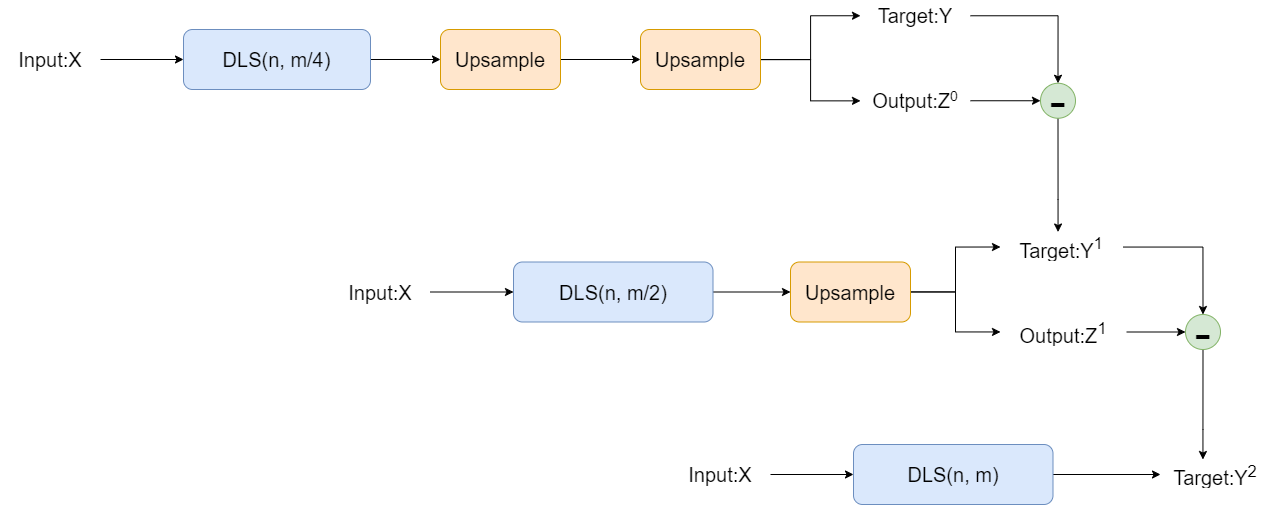
\includegraphics[width=0.8\textwidth]{DLS_Resnet.png} 
\caption{Resnet结构}
\end{figure}

暂时模型的残差网络结构如上,还在改进中,coming soon...

\section*{4. 模型测试}
由于模型仍在改进,这里暂时我们只在电力和交通数据集上做了评测,可以看出加上Resnet的DLS模型在两个数据集上都获得了更低的mae和mse,这也证明了该模型的有效性。

\begin{figure}[H]
\centering 
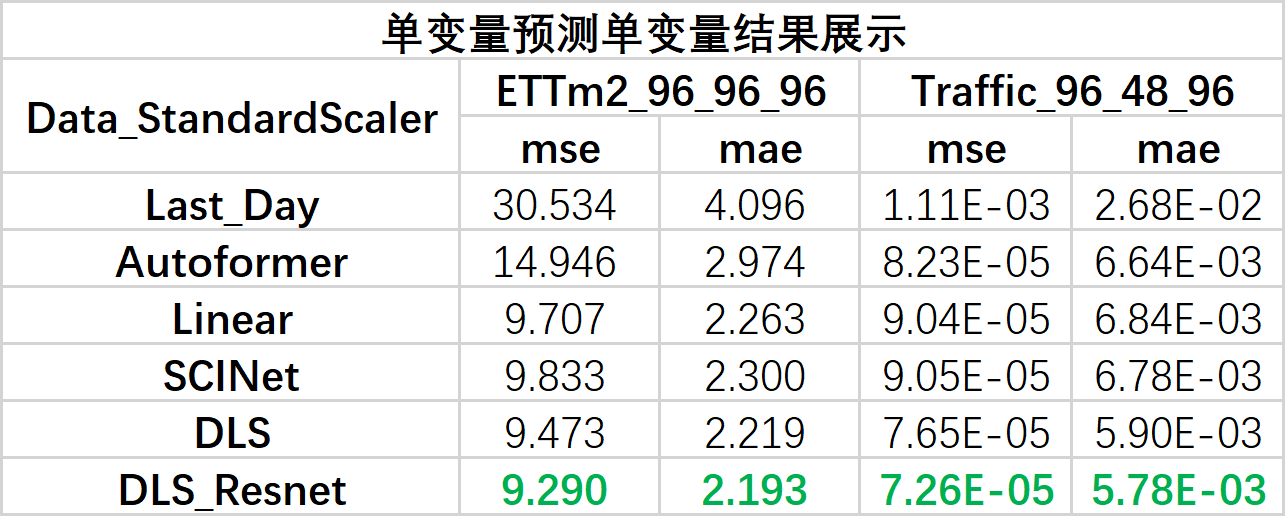
\includegraphics[width=0.8\textwidth]{1.png} 
\caption{暂时模型测试结果,更多结果coming soon...}
\end{figure}

\begin{figure}[H]
\centering  %图片全局居中
\subfigure[模型DLSResnet的预测结果]{
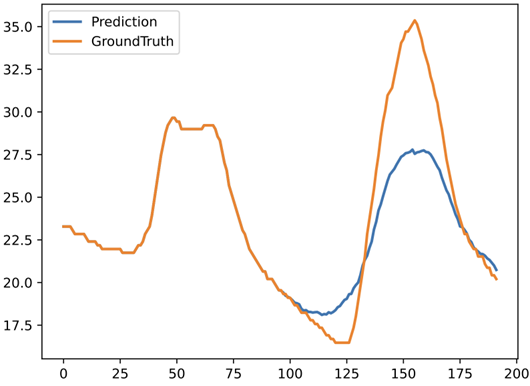
\includegraphics[width=0.4\textwidth]{2.png}}
\subfigure[模块DLS(n,m/4)的预测结果]{
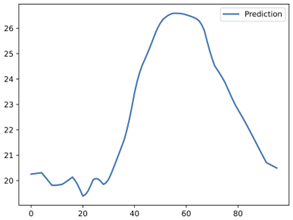
\includegraphics[width=0.4\textwidth]{2_1.png}}
\subfigure[模块DLS(n,m/2)的预测结果]{
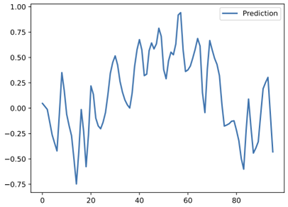
\includegraphics[width=0.4\textwidth]{2_2.png}}
\subfigure[模块DLS(n,m)的预测结果]{
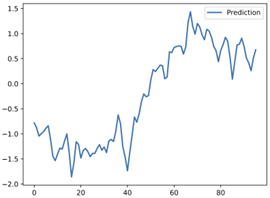
\includegraphics[width=0.4\textwidth]{2_3.png}}
\caption{模型DLSResnet在ETTm2上的预测结果。a图是整个模型的预测结果,b、c、d是模型的三个模块的预测结果。}
\end{figure}

\begin{figure}[H]
\centering  %图片全局居中
\subfigure[模型DLSResnet的预测结果]{
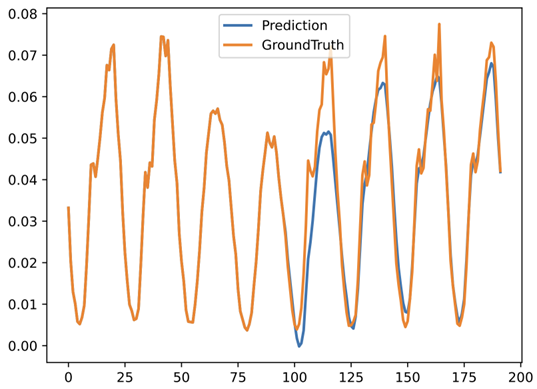
\includegraphics[width=0.4\textwidth]{3.png}}
\subfigure[模块DLS(n,m/4)的预测结果]{
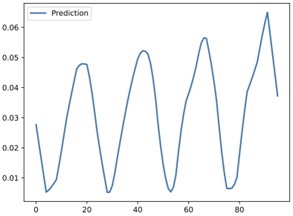
\includegraphics[width=0.4\textwidth]{3_1.png}}
\subfigure[模块DLS(n,m/2)的预测结果]{
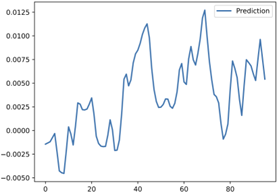
\includegraphics[width=0.4\textwidth]{3_2.png}}
\subfigure[模块DLS(n,m)的预测结果]{
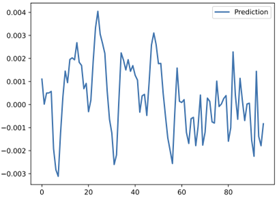
\includegraphics[width=0.4\textwidth]{3_3.png}}
\caption{模型DLSResnet在Traffic上的预测结果。a图是整个模型的预测结果,b、c、d是模型的三个模块的预测结果。}
\end{figure}

\end{document}

%%% Local Variables: 
%%% mode: latex
%%% TeX-master: t
%%% End: 
